\graphicspath{{}{miniboone/figs/}{miniboone/}}

\textbf{Introduction --} Non-zero neutrino masses have been established in the last twenty years by measurements of neutrino flavor conversion in natural and human-made sources, including long- and short-baseline experiments. The overwhelming majority of data points towards a three-neutrino framework. Within this framework, we have measured the mixing angles that parametrize the relationship between mass and flavor eigenstates to percent-level precision~\cite{Esteban:2018azc}. The remaining unknowns are the absolute scale of neutrino masses and their origin, the CP-violating phase, and the mass ordering of the neutrinos. In addition, anomalies in short-baseline accelerator and reactor experiments~\cite{Athanassopoulos:1996jb,Aguilar:2001ty,AguilarArevalo:2007it,Aguilar-Arevalo:2018gpe} are yet to have satisfying explanations. The most significant anomalies are beyond statistical doubt. Minimal extensions of the three-neutrino framework to explain the anomalies introduce the so-called sterile neutrino states, which do not participate in Standard Model (SM) interactions in order to agree with measurements of the Z-boson invisible decay width~\cite{ALEPH:2010aa}. Unfortunately, these minimal scenarios are disfavoured as they fail to explain all data~\cite{Collin:2016aqd, Capozzi:2016vac, Dentler:2018sju}. This has led the community to explore nonminimal scenarios. Along this direction, it is interesting to study well-motivated neutrino-mass models that can also explain the short-baseline anomalies and are testable in the laboratory. In this work, we will examine the class of neutrino-mass-related models that have been proposed as an explanation of the anomalous observation of electron-neutrino-like events in MiniBooNE~\cite{Aguilar-Arevalo:2018gpe}.

The MiniBooNE excess is currently in tension with the standard three-neutrino prediction at a level of $4.7 \sigma$~\cite{Aguilar-Arevalo:2018gpe}. While it is possible that the excess is fully or partially due to systematic uncertainties or SM backgrounds~(see, \textit{e.g.},~\cite{AguilarArevalo:2008rc,Aguilar-Arevalo:2012fmn,Hill:2010zy}), many Beyond the Standard Model (BSM) explanations have been put forth. These new physics (NP) scenarios typically require the existence of new particles, which can: participate in short-baseline oscillations~\cite{Murayama:2000hm,Strumia:2002fw,  Barenboim:2002ah, GonzalezGarcia:2003jq, Barger:2003xm,Sorel:2003hf, Barenboim:2004wu, Zurek:2004vd, Kaplan:2004dq, Pas:2005rb, deGouvea:2006qd,Schwetz:2007cd, Farzan:2008zv, Hollenberg:2009ws,Nelson:2010hz, Akhmedov:2010vy, Diaz:2010ft, Bai:2015ztj, Giunti:2015mwa, Liao:2016reh, Papoulias:2016edm, Moss:2017pur, Carena:2017qhd}, change the neutrino propagation in matter~\cite{Liao:2016reh, Liao:2018mbg,Asaadi:2017bhx,Doring:2018cob}, be produced in the beam or in the detector and its surroundings~\cite{Gninenko:2009ks,Gninenko:2010pr,Dib:2011jh,McKeen:2010rx,Masip:2012ke, Masip:2011qb,Gninenko:2012rw,Magill:2018jla}. These models either increase the conversion of muon- to electron-neutrinos or produce electron-neutrino-like signatures in the detector, where in the latter category one typically exploits the fact that the LSND and MiniBooNE are Cherenkov detectors that cannot distinguish between electrons and photons. Although it is possible to consider MiniBooNE explanations that have little to no theoretical motivation, recent models~\cite{Bertuzzo:2018itn,Bertuzzo:2018ftf,Ballett:2018ynz} are motivated by neutrino-mass generation via hidden interactions in the heavy neutrino sector. In particular, the common feature of these models is the upscattering into a heavy neutrino, usually with tens to hundreds of MeV in mass, which subsequently decays into a pair of electrons. If collimated, this pair of electrons can fake a single-electron signature.

In this article, we introduce new techniques to probe these testable neutrino mass generation models in past, present, and future neutrino experiments. In addition, our analysis showcases a generic way to look for models that rely on the ambiguity between photons and electrons to explain the MiniBooNE observation. Due to the electron-like nature of the excess, we consider neutrino-electron scattering measurements~\cite{Auerbach:2001wg, Deniz:2009mu,Bellini:2011rx,Park:2013dax,Vilain:1994qy}. Although these experiments have been shown to provide powerful constraints on light NP~\cite{Pospelov:2017kep,Lindner:2018kjo,Magill:2018tbb}, the unique topology of the signatures we consider requires us to go beyond the final processed sample quoted by the experiments and develop new ways to search for them.
Since the typical heavy neutrino mass is in the hundreds-of-MeV regime, we focus on two high-energy neutrino experiments: \minerva~\cite{Park:2013dax,Park:2015eqa,Valencia-Rodriguez:2016vkf} and CHARM-II~\cite{DeWinter:1989zg,Geiregat:1992zv,Vilain:1994qy}. These experiments are complementary in neutrino energy and background composition. In both cases we make use of sideband measurements, taking advantage of the excellent particle reconstruction capabilities of \minerva and the precise measurements at CHARM-II to constrain NP.
%
%%% DIAGRAM %%%
\begin{figure}[t!]
    \centering
    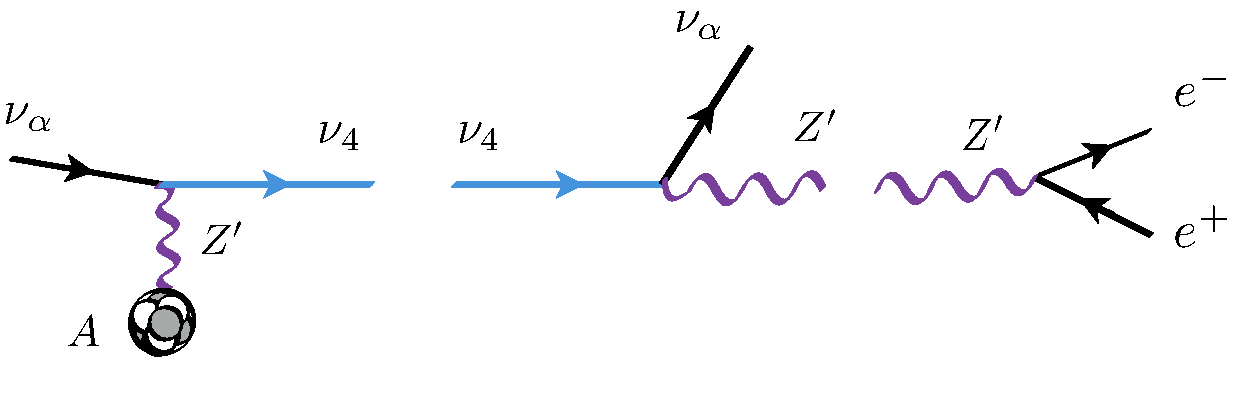
\includegraphics[width=0.65\textwidth]{diagram.pdf}
    \caption[Dark neutrino signal at MiniBooNE.]{{\textit{Illustration of heavy neutrino production.}} Left: production of the heavy mass state via upscattering. Center: Decay of the heavy neutrino into a light neutrino and a gauge boson. Right: Decay of a gauge boson into a pair of electrons that produce the experimental signature.\label{fig:diagram}}
\end{figure}

%%%%%%%%%%%%%%%%%%%%%%%%%
\textbf{Model --} We limit our discussion to the minimal version of the model that could explain the MiniBooNE excess. This contains at least one heavy neutrino, $\nu_D$, charged under a new U$(1)^\prime$ gauge group, which is part of the particle content and gauge structure needed for mass generation. The $\nu_D$ can be either of a Dirac or Majorana~\cite{Bertuzzo:2018ftf} nature. In this paper, we show our results for a Dirac particle since the Majorana case is more severely in tension with the angular distribution~\cite{Formaggio:1998zn,Balantekin:2018ukw}. The dark sector is connected to the SM in two ways: through kinetic mixing between the new gauge boson and hypercharge, and through neutrino mass mixing. We start by specifying the kinetic part of the NP Lagrangian
%
\begin{equation}
\mathscr{L}_{\rm kin} \supset
\;\; \frac{1}{4} \hat{Z}^{\prime}_{\mu \nu} \hat{Z}^{\prime \mu \nu} + \frac{\sin{\chi}}{2} \hat{Z}^{\prime}_{\mu \nu} \hat{B}^{\mu \nu} + \frac{m_{\hat{Z}^\prime}^2}{2} \hat{Z}^{\prime \mu} \hat{Z}^\prime_{\mu},
\end{equation}
%
where $\hat{Z}^{\prime \mu}$ stands for the new gauge boson field, $\hat{Z}^{\prime \mu\nu}$ its field strength, and $\hat{B}^{\mu \nu}$ the hypercharge field strength. After usual field redefinitions~\cite{Chun:2010ve}, we arrive at the physical states of the theory. Working at leading order in $\chi$ and assuming $m_{Z^\prime}^2/m_{Z}^2$ to be small, we can specify the relevant interaction Lagrangian as
%
\begin{equation}
\mathscr{L}_{\rm int} \supset \;\;g_D \overline{\nu}_D \gamma_\mu \nu_D Z^{\prime \mu}
 + e \varepsilon Z'^{\mu}J^{\rm EM}_{\mu},
\end{equation}
%
where $J^{\rm EM}_{\mu}$ is the SM electromagnetic current, $g_D$ is the U$(1)^\prime$ gauge coupling assumed to be $\mathcal{O}(1)$, and $\varepsilon \equiv c_{\rm w} \chi$, with $c_{\rm w}$ being the cosine of the weak angle. Additional terms would be present at higher orders in $\chi$ and mass mixing with the SM $Z$ is also possible, though severely constrained. 
After electroweak symmetry breaking, the dark neutrino $\nu_D$ is a superposition of neutrino mass states. The flavor and mass eigenstates are related via 
\begin{equation}
    \nu_\alpha = \sum^{4}_{i=1} U_{\alpha i}\nu_{i}, \quad (\alpha=e,\mu,\tau,D),
\end{equation}
where $U$ is a $4\times4$ unitary matrix. It is expected that $|U_{\alpha 4}|$ is small for $\alpha = e, \mu, \tau$, but $|U_{D4}|$ can be of $\mathcal{O}(1)$~\cite{Parke:2015goa,Collin:2016aqd}. The choice of $m_4$ and $m_{Z^\prime}$ has important consequences for the allowed decays of the new particle content. We focus on the case in which $m_4 > m_{Z^\prime}$, where the two body $\nu_4 \to \nu_\alpha Z^\prime$ decay is allowed. In addition, the mass of the new gauge boson is kept below $\sim100$ MeV, making the decay into $e^+e^-$ pairs the dominant channel. Decay into a pair of neutrinos is possible, but is subdominant provided the mixing is small. 
%
%%%%%%%%%%%%% Cross Section %%%
\begin{figure}[t!]
    \centering
    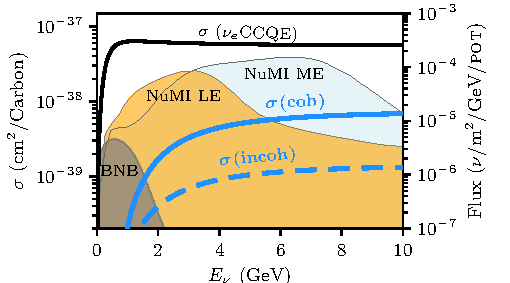
\includegraphics[width=0.49\textwidth]{cross_sections.pdf}
    \caption[Upscattering total cross section.]{{\textit{Upscattering cross section compared to the quasi-elastic.}} The quasi-elastic cross section for $6p^+$ is shown as a function of the neutrino energy (solid black line). Similarly the coherent, out of a carbon atom, and the diffractive NP contributions for the benchmark point of~\cite{Bertuzzo:2018itn} are shown as solid and dashed blue lines, respectively. In the background, the light gray shaded region is the Booster Neutrino Beam (BNB) flux shape, while the light golden region is the Neutrinos at the Main Injector (NuMI) low-energy neutrino-mode flux.}{\label{fig:cross_section}}
\end{figure}
%%%%%%%%%%%%%%%%%%%%%%%%%%%%%%%%%%%%%%%%%%%%%%%%%%

\textbf{Signature --} As illustrated in Fig.~\ref{fig:diagram}, the heavy neutrino is produced by upscattering from an active neutrino flavour state. The production cross section is proportional to $ \alpha_D \alpha_{\rm QED} \varepsilon^2 |U_{\alpha 4}|^2$, usually dominated by the muon-neutrino contribution due to the flavor composition of the beam. This production can happen off the whole nucleus in a coherent way or off individual nucleons. For $m_{Z^\prime} \lesssim 100$ MeV, the production will be mainly coherent, but for heavier masses, such as the ones considered in~\cite{Ballett:2018ynz}, the upscattering happens predominantly in a diffractive regime. In Fig.~\ref{fig:cross_section}, we show the cross section at the benchmark point of~\cite{Bertuzzo:2018ftf} and compare it with the quasi-elastic cross section. By superimposing the cross section on the neutrino fluxes of \minerva and MiniBooNE, we make it explicit that the larger energies at \minerva and CHARM-II are ideal to probe these models. Once produced, $\nu_4$ is then expected to decay promptly inside of the detector, setting a requirement on its lifetime. The mass of the heavy neutrino also controls the angular distribution of the signal with respect to the beam. The lighter $\nu_4$ is, the more forward the signal will be.
The produced $Z^\prime$ is required to decay into an overlapping $e^+e^-$ pair, setting a lower bound on its mass of a few MeV.
To summarize, increasing $m_{Z^\prime}$ has two effects. On one hand, it increases the ratio of diffractive to coherent upscattering, and on the other hand, it makes the electron pair less collimated. 
Even though we focus on overlapping $e^+e^-$ pairs, we note that a significant fraction of events would appear as well-separated electrons or as a pair of electrons with large energy asymmetry, similarly to the neutral current $\pi^0$ events. The asymmetric events also contribute to the MiniBooNE excess and can also be looked for in $\nu-e$ scattering analyses.

{\bf Analysis --} Neutrino-electron scattering measurements at \minerva and CHARM-II predicate their cuts in the following core ideas: no hadronic activity near the interaction vertex, small opening angle from the beam, $E_e \theta^2 < 2 m_e$, and the requirement that the measured energy deposition $dE/dx$ be consistent with that of a single electron. When the coherent process dominates and the mass of the $Z^\prime$ is small, the first two conditions are satisfied. However, the requirement of a single-electron-like energy deposition removes a significant fraction of the new-physics induced events. This presents a challenge, as the signal events are mostly overlapping electron pairs and will potentially be removed by the $dE/dx$ cut.
In order to circumvent this problem, we do our analysis not at the final-cut level, but at an intermediate one. The CHARM-II experiment provides data as a function of $E_e \theta^2$ without the $dE/dx$ cut, and in the case of \minerva we have access to the data as a function of the measured $dE/dx$ after analysis cuts on $E_e \theta^2$.

We briefly describe the main features of the \minerva event selection here (for more details see~\cite{Park:2015eqa}). The minimum electron energy required is $0.8$ GeV in order to remove the $\pi^0$ background and have reliable angular and energy reconstruction. Events are kept only when they meet the following angular separation criterion: $E_e \theta^2 < 3.2\times 10^{-3}~{\rm ~GeV ~rad^2}$. A final cut is applied, ensuring $dE/dx < 4.5~{\rm MeV} / 1.7~{\rm cm}$. The \minerva analysis uses the data outside the previous $dE/dx$ cut to contrain backgrounds. This sideband is defined as all events with $E_e\theta^2 > 5 \times 10^{-3} {\rm ~GeV ~rad^2}$ and $dE/dx < 20~{\rm MeV}/1.7~{\rm cm}$. Using this sideband measurement, the collaboration tunes their backgrounds by (0.76, 0.64, 1.0) for ($\nu_e$CCQE, $\nu_\mu$NC, $\nu_\mu$CCQE) processes. 
We perform our analysis with the data shown in Fig. 3 of~\cite{Park:2015eqa} where all the cuts are applied except for the final $dE/dx$ cut. We have developed our own Monte Carlo (MC) to simulate candidate electron pair events; in our MC simulation, detector-resolution effects are assumed to be Gaussian with appropriate widths taken from~\cite{Aliaga:2013uqz}. We only consider the coherent part of the cross section to avoid hadronic-activity cuts, which is conservative. We also select only events with small energy asymmetries and small opening electron angles. We calculate the mean $dE/dx$ in plastic scintillators~\cite{NIST:2018} according to~\cite{Leo:1987kd,Tanabashi:2018oca}. 
In our final event selection, we require that the sum of the energy deposited by each electron be more than $4.5$ MeV$/ 1.7$ cm, which yields an efficiency of $90\%$. We obtain the expected size of neutrino-electron scattering and background events in this range from Fig. 3 of~\cite{Park:2015eqa}. To place our limits, we perform a rate-only analysis by means of a $\chi^2$ test statistic. We incorporate uncertainties in background size and flux normalization as nuisance parameters with Gaussian constraint terms. For the neutrino electron scattering and BSM signal, we allow the normalization to scale proportionally to the same flux uncertainty parameter. 
The background term also scales with the flux-uncertainty parameter but has an additional nuisance parameter to account for its unknown size. We obtain our constraint as a function of heavy neutrino mass $m_4$, and mixing $|U_{\mu 4}|$ assuming with two degrees of freedom~\cite{Tanabashi:2018oca}.
In our nominal \minerva analysis, we allow for 30\% uncertainty on the background motivated by the amount of tuning performed on the original backgrounds. Note that the nominal background predictions in the \minerva analysis overpredicts the data before tuning, and that tuning parameters are measured at the 3\% level~\cite{Park:2013dax}.
We also perform a background-ignorant analysis in which we assume 100\% uncertainty for the background normalization, which changes our conclusions by only less than a factor of two. This emphasizes the robustness of our \minerva bound, since the NP typically overshoots the low number of events in the sideband.



\section{Using neutrino-electron scattering data}

\begin{figure}
 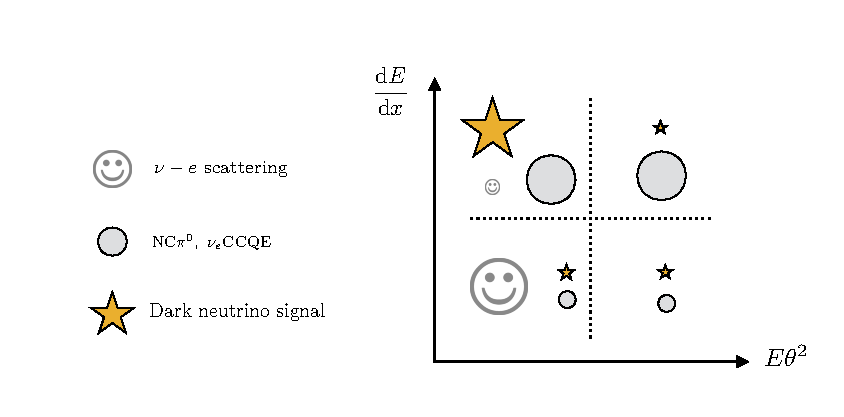
\includegraphics[width = 0.8\textwidth]{MiniBooNE_tests.pdf}
 \caption[Diagram of the sidebands in neutrino-electron scattering analyses.]{A schematic representation of the relative number of events in sideband regions of neutrino-electron scattering analyses.}
\end{figure}


Our CHARM-II analysis is mostly based on Fig. 1 of~\cite{Vilain:1994qy}. This sample is shown as a function of $E\theta^2$ and does not have any cuts on $dE/dx$. The NP signal lies mostly in a region with small $E\theta^2$. Thus, we constrain backgrounds using the data from $30 < E\theta^2 < 60$ MeV rad$^2$. This sideband measurement constrains the normalization of the backgrounds in the signal region at the level of $3\%$.
The extrapolation of the shape of the background to the signal region introduces the largest uncertainty in our analysis. For this reason, we raise the uncertainty of the background normalization from $3\%$ to a conservative $10 \%$ when setting the limits. Flux uncertainties are assumed to be $4\%$~\cite{Allaby:1987bb} and are applicable to the new-physics signal, $\nu-e$ scattering prediction, and backgrounds. 
Our $\chi^2$ test is similar to the one used in the \minerva analysis and carries normalization nuisance parameters for the background and flux predictions. Uncertainties in the $\nu-e$ scattering cross sections are expected to be sub-dominant and are neglected in the analysis~\cite{deGouvea:2006hfo}.

We have performed our own fit to the MiniBooNE energy spectrum using the data release from~\cite{Aguilar-Arevalo:2018gpe}, and our results agree with~\cite{Bertuzzo:2018itn}. The data release, however, only contains information about the neutrino energy and baseline distance. Thus, the re-weighting procedure for the model of interest can only be performed approximately. A proper analysis can be performed only if true and reconstructed electron angles and energies per simulated event are given.  

%
\begin{figure}[t]
    \centering
    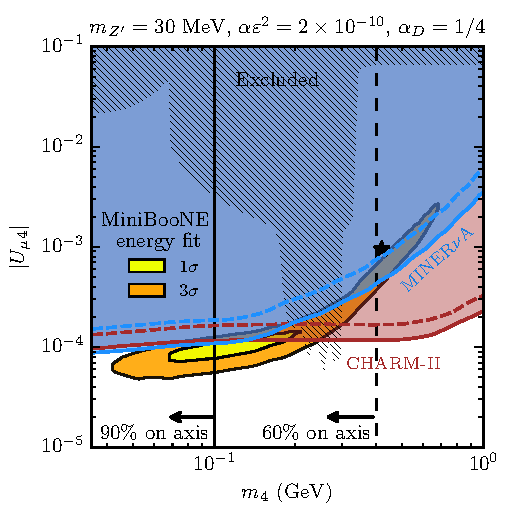
\includegraphics[width=3.38in]{bounds.pdf}
    \caption[New constraints on dark neutrinos.]{{\textit{New constraints on mass generation model as a MiniBooNE explanation.}} The MiniBooNE region of interest from~\cite{Bertuzzo:2018itn}, only fitted to the energy distribution, is shown as closed yellow (orange) regions for one (three) sigma C.L. The benchmark point, chosen to provide a good angular distribution fit, is shown as a black star. Exclusion from heavy neutrino searches is shown as a hatched background. Our new constraints at 90\% C.L. using \minerva are shown in blue for our nominal 30\% background normalization uncertainty (solid) and conservative case of 100\% background uncertainty (dashed). Our CHARM-II bound is shown in cherry red, where the 3\% background normalization from the sideband is shown as a solid curve and the conservative 10\% case as a dashed curve. The solid vertical black line at 100 MeV signals the point where 90\% of NP events lie in the most forward bin in the MiniBooNE angular distribution, and the dashed one where 60\% of events do so. Other relevant assumed parameters are shown above the plot; changing them does not change our conclusion.}
    \label{fig:final_plot}
\end{figure}
%

{\bf Results and conclusions --}
The resulting limits at 90\% confidence level (CL)  in the $|U_{\mu 4}|$ vs $m_4$ plane are shown in~\reffig{fig:final_plot}, together with the MiniBooNE fit from~\cite{Bertuzzo:2018itn}. For comparison, we have chosen the same values of $\varepsilon$, $\alpha_D$, and $m_{Z^\prime}$ as used in~\cite{Bertuzzo:2018itn}. 
We note that the MiniBooNE event rate scales identically to our signal rate in all the couplings, and the dependence of our bounds on $m_{Z^\prime}$ is subleading due to the large $Q^2$ involved. 
This implies that changing the values of these parameters does not modify the overall conclusions of our work. In addition, one can lower the value of $m_{Z^\prime}$ to only around $10$ MeV before hitting beam dump constraints~\cite{Bauer:2018onh}. 
On the other hand, for this realization of the model, larger $m_{Z^\prime}$ implies larger values of $m_4$, increasing the tension between the MiniBooNE fit and our bounds.
Our results from \minerva and CHARM-II are compatible given that 
they impose similar constraints for $m_4 \lesssim 200 $ MeV. For larger masses, the kinematics of the signal becomes less forward and the production thresholds start being important. This explains the upturns visible in our bounds, where we observe it first in \minerva and later in CHARM-II as we increase $m_4$, since CHARM-II has higher beam energy and the neutrino flux peaks at approximately 20 GeV.

The preferred region of~\cite{Bertuzzo:2018itn} results from doing an energy-spectrum only fit to the MiniBooNE data. This neglects the angular distribution of the MiniBooNE excess. The preferred region of this energy-only fit is excluded by our analysis for masses of $m_4$ greater than $\approx 250$ MeV. As was recently pointed out in~\cite{Jordan:2018qiy}, reasonable angular distribution of NP explanations of the MiniBooNE excess requires hundreds of MeV NP particles.
Since the released MiniBooNE data do not provide the correlation between angle and energy and their associated systematics, a rigorous assessment of the tension is hard to quantify. The angular distribution of observed excess contains $\approx 50\%$ of the events in the most forward bin, with a statistical uncorrelated uncertainty of 5\% on this quantity.
We use this information and our calculation of the angular distribution of the NP events from our dedicated MC to give an assessment of the tension in this observable. We draw a vertical line at $m_4 = 100$ MeV, where 90\% of the NP events would lie in the most forward bin and a dashed line at 60\%. 
This 60\% line, as expected, is close to the benchmark point of~\cite{Bertuzzo:2018ftf}. This consideration suggests that our analysis targets precisely the region where the model can lead to agreement in the angular data. 

In the near future, the \minerva medium-energy results on neutrino-electron scattering will be available. With the increase in energy, we estimate that it can improve the probe significantly if backgrounds, which are also rising, are well understood.
This class of analyses will thus greatly benefit from improved calculations and measurements of coherent $\pi^0$ production and single-photon emitting processes. This is particularly important if an excess is observed in these channels.
A complementary result can also be obtained by measuring this process in NO$\nu$A, which will sample a different kinematic regime as its off-axis beam peaks at lower energies and expects fewer NC$\pi^0$ events per ton. 
Interestingly, we note that this class of BSM signatures could be lurking in current measurements of $\pi^0$ production, \textit{e.g.}, at MINOS~\cite{Adamson:2016hyz} and MINER$\nu$A~\cite{Wolcott:2016hws}. The latter measurement observes a significant excess of diffractive events, which are abundant in similar realizations of this NP model~\cite{Ballett:2018ynz}.
To summarize, a variety of measurements are underway to further lay siege to this explanation of the MiniBooNE observation and, simultaneously, start probing testable neutrino mass generation models, as well as other similar NP signatures. It is clear that understanding neutrino cross sections will be crucial as we move forward.
